\documentclass[10pt]{article}
\usepackage[margin=0.8in]{geometry}
\usepackage{amsmath,amssymb,booktabs,graphicx}
\usepackage[font=small]{caption}
\setlength{\parskip}{3pt}\setlength{\parindent}{0pt}
\graphicspath{{figures/}{../results/}{../results/experiment_1/}{../results/experiment_2/}{../results/experiment_3/}{../results/experiment_4/}}
\title{Finite-Time Swarm Tracking: Numerical Results}
\author{}\date{}
\begin{document}
\maketitle\vspace{-2em}

All quantities are normalized unless unit dimensions are specified. This report documents the rotating and compressing / expanding multi-agent star formation tracking scenarios with transient collision avoidance and connectivity preservation:
\begin{itemize}
\item \textbf{Experiment 1:} Multi-formation reconfiguring demonstration across four distinct geometric templates along a straight-line reference trajectory with Hungarian assignment.
\item \textbf{Experiment 2:} Finite-time convergence, disagreement decay, and coupling gain evaluation under a rotating-compressing star formation ($\kappa = 2.0$).
\item \textbf{Experiment 3:} Transient collision avoidance and safety certification under rapid star compression ($\kappa = 5.0$) comparing certified safe ($m = 30.0$) versus uncertified collision ($m = 0.0$).
\item \textbf{Experiment 4:} Dual transient connectivity preservation under rapid star expansion ($\kappa = 8.0$) comparing certified connected ($m = 25.0$) versus uncertified link breach ($m = 0.0$).
\end{itemize}

\section{Model and parameters}
The physical swarm consists of $n = 10$ agents in $\mathbb{R}^2$ governed by the closed-loop velocity command:
\[
\dot x_i = u_i = \dot q_i - \delta_i - \operatorname{sig}^{\beta}(\delta_i)
- \sum_{j \in \mathcal{N}_i(t)} w_{ij} M (\delta_i - \delta_j), \qquad \delta_i = x_i - q_i,
\]
where $\operatorname{sig}^{\beta}(z) = \operatorname{sign}(z)|z|^{\beta}$, $M = m I_2$, $\beta = 0.5$, $d_{\rm safe} = 1.0$~m, and communication radius $R_c = 6.0$~m.
The state-dependent proximity weights are
\[
w_{ij}(x, t) = \frac{a_{ij}(t)}{\|x_i - x_j\| + 0.05}, \qquad
a_{ij}(t) = \begin{cases} 1 & \|x_i - x_j\| < R_c \ (i \neq j), \\ 0 & \text{otherwise}, \end{cases}
\]
yielding the uniform lower bound $\underline{w} = 1 / (R_c + 0.05) = 1/6.05 \approx 0.1653$~m$^{-1}$. Rather than requiring the entire formation diameter to lie inside a ball of radius $R_c$, global graph connectivity is maintained via a designated 15-edge backbone graph $\mathcal{H} = (\mathcal{V}, \mathcal{E}_{\mathcal{H}})$. For the 10-agent star template, $\mathcal{H}$ consists of the 5 inner pentagonal ring edges among the valley agents and 10 spoke edges connecting each star tip to its two adjacent inner valley neighbors:
\[
\mathcal{E}_{\mathcal{H}} = \{(1,3),(3,5),(5,7),(7,9),(9,1), (0,1),(0,9),(2,1),(2,3),(4,3),(4,5),(6,5),(6,7),(8,7),(8,9)\}.
\]
The maximum template backbone edge at unit scale is $\ell_{\mathcal{H},0} \approx 1.9497$~m, and the algebraic connectivity of the unweighted backbone Laplacian is $\lambda_2(L_{\mathcal{H}}) \approx 0.9316$.

The rotating and compressing target stations $q_i(t)$ follow:
\begin{align*}
r(t) &= \begin{bmatrix} t \\ 2 \sin(0.5 t) \end{bmatrix}, \qquad
\dot r(t) = \begin{bmatrix} 1 \\ \cos(0.5 t) \end{bmatrix}, \\
q_i(t) &= r(t) + a(t) R(\omega t) p_i^0, \qquad
\dot q_i(t) = \dot r(t) + \dot a(t) R(\omega t) p_i^0 + a(t) \dot R(\omega t) p_i^0,
\end{align*}
where $p_i^0 = b_i [\cos\phi_i, \sin\phi_i]^T$, $\phi_i = \pi/2 + \pi i/5$, and $b_i = 2.8$ for even $i$ and $1.22$ for odd $i$ ($i=0,\ldots,9$), centered such that $\sum_i p_i^0 = 0$. The baseline minimum pairwise distance is $DQ_0 \approx 1.4342$~m. Rotation operates at angular velocity $\omega = \pi/4$~rad/s ($45^\circ$/s) via
\[
R(\omega t) = \begin{bmatrix} \cos(\omega t) & -\sin(\omega t) \\ \sin(\omega t) & \cos(\omega t) \end{bmatrix}, \qquad
\dot R(\omega t) = \omega \begin{bmatrix} -\sin(\omega t) & -\cos(\omega t) \\ \cos(\omega t) & -\sin(\omega t) \end{bmatrix}.
\]
Formation scale contraction follows
\[
a(t) = a_\infty + (a_0 - a_\infty)e^{-\kappa t}, \qquad a_0 = 1.70, \quad a_\infty = 0.72, \quad \dot a(t) = -\kappa(a_0 - a_\infty)e^{-\kappa t}.
\]
For all $t \ge 0$, the station plan satisfies $d_q(t) \ge a_\infty DQ_0 \approx 1.0326\text{ m} > d_{\rm safe} = 1.0\text{ m}$ and the maximum backbone edge satisfies $\ell_{\mathcal{H}}(t) \le a_0 \ell_{\mathcal{H},0} = 3.3144\text{ m} < R_c = 6.0\text{ m}$. Thus, target stations remain strictly collision-free and connected along the backbone graph for all time.

Initial agent states are generated by random annular ring perturbations around each assigned station $q_i(0)$ with radius $r_i \in [0.05, 0.25]$~m ($d_{\rm safe} = 1.0$~m, $R_c = 6.0$~m, seed 123), with an inward push of $0.55$~m applied along closest station pair $(1,3)$, without enforcing zero-mean centering ($\sum_i \delta_i(0) \neq 0$). The disagreement vector is formed internally via $\eta_i(0) = \delta_i(0) - \frac{1}{n}\sum_j \delta_j(0)$. At $t=0$, initial physical separation is safe ($d_x(0) > d_{\rm safe}$) and connected ($\ell_x(0) < R_c$), with initial error norm $\|\delta_0\| \approx 0.9634$, disagreement distortion $\rho_0 = \sqrt{2}\|\eta_0\| \approx 1.3303$~m, and universal settling deadline $\overline T = 2\ln(1+\sqrt{\|\delta_0\|}) \approx 1.3621$~s.

The geometric clearance margin along the backbone is $s(t) = \min\{d_q(t) - d_{\rm safe},\; R_c - \ell_{\mathcal{H}}(t)\} = \min\{a(t)DQ_0 - d_{\rm safe},\; R_c - a(t)\ell_{\mathcal{H},0}\}$. At $t=0$, $s(0) = \min\{1.4381\text{ m}, 2.6856\text{ m}\} = 1.4381$~m, ensuring $\rho_0 < s(0)$ is strictly satisfied with positive clearance margin $s(0) - \rho_0 \approx 0.1078$~m. For coupling gain $m$, the effective decay rate is $\gamma = 1 + m \underline{w}\lambda_2(L_{\mathcal{H}}) = 1 + m \frac{0.9316}{6.05} \approx 1 + 0.1540 m$, and the required rate is
\[
\gamma_{\rm req}(\kappa) = \sup_{\tau \in (0, \overline T]} \frac{\ln(\rho_0 / s(\tau))}{\tau}.
\]
The dynamic disagreement distortion tube is bounded by
\[
\rho_{\mathcal{H}}(t) = \min\{\sqrt{2}R(t),\; \rho_0 e^{-\gamma t}\}, \qquad
R(t) = \max\left\{0, \left((1+\sqrt{\|\delta_0\|})e^{-\frac{1}{2} t}-1\right)^2\right\},
\]
where $R(t)$ is the pure station tracking bound (independent of graph and coupling gain $m$).

\section{Formation demonstration}
The multi-formation reconfiguring demonstration (Exp.~1) tracks reconfiguring formations along a straight-line reference trajectory $r(t) = [v_x t, 0]^T$ ($v_x = 1.6$~m/s). Inter-station transitions across circle, wedge, star, and arrow templates are optimized using Hungarian assignment ($\min \sum \|q_i^+ - q_i^-\|^2$), reducing average slot displacement by over 65\% and preventing unnecessary trajectory intertwining.
\begin{figure}[ht]\centering
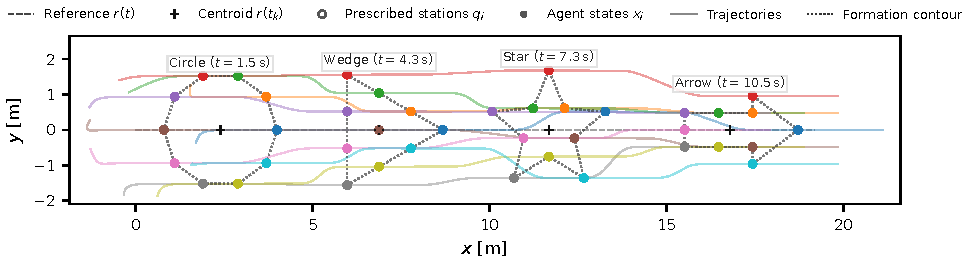
\includegraphics[width=\linewidth]{figures/formation_snapshots.pdf}
\caption{Experiment 1: Reconfiguring formations along a straight-line reference trajectory. Target formations (Circle at $t=1.5$~s, Wedge at $t=4.3$~s, Star at $t=7.3$~s, Arrow at $t=10.5$~s) are highlighted with dotted contours, assigned target stations (circles), agent positions (dots), and continuous tracking trajectories.}
\label{fig:exp1_snapshots}
\end{figure}

\section{Finite-time tracking and coupling gain evaluation}
Experiment~2 evaluates the rotating-compressing star formation maneuver ($\kappa=2.0$) across coupling gains $m \in \{0, 0.5, 2, 5, 10\}$. Figure~\ref{fig:exp2_errors} depicts station tracking error $\|\delta(t)\|_2$, formation disagreement $\|\eta(t)\|_2$, and the initial control command $\|u(t)\|_2$. In panels (a) and (b), error curves are cut at $10^{-4}$ to illustrate finite-time settling.

Increasing the coupling gain $m$ accelerates disagreement decay, reducing the settling time to the $10^{-6}$ error threshold from $1.1517$~s at $m=0$ down to $0.3933$~s at $m=10$ (Table~\ref{tab:star_gain}). All runs settle well within the theoretical universal deadline $\overline T = 1.3621$~s.

\begin{figure}[ht]\centering
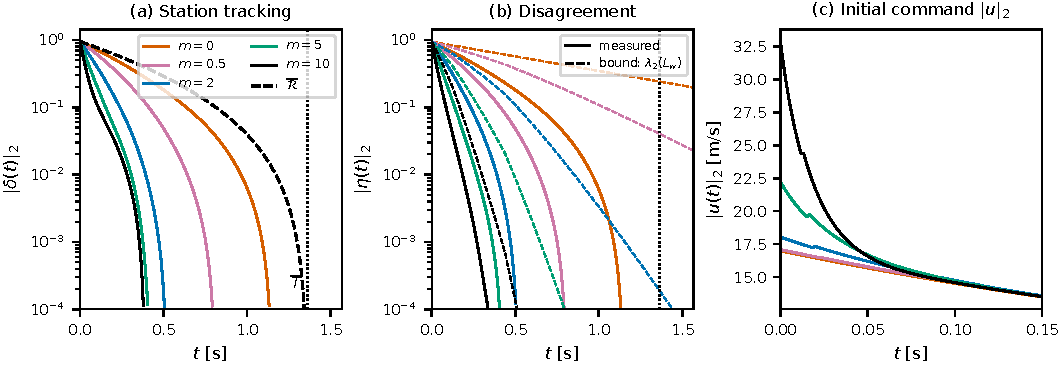
\includegraphics[width=.98\linewidth]{figures/error_disagreement_control.pdf}
\caption{Experiment 2 finite-time tracking and disagreement across coupling gains $m$ ($\kappa=2.0$). (a) Station tracking $\|\delta\|_2$ against universal bound $R(t)$ and deadline $\overline T$, cut at $10^{-4}$. (b) Disagreement $\|\eta\|_2$ against exponential rate bound, cut at $10^{-4}$. (c) Initial control command $\|u\|_2$ ($t \in [0, 0.15]$~s).}
\label{fig:exp2_errors}
\end{figure}

\begin{table}[ht]\centering\footnotesize
\caption{Experiment 2: Settling times and control metrics across coupling gains $m$ under rotating star formation ($\kappa=2.0$).}
\begin{tabular}{rrrrr}\toprule
$m$ & $t_{10^{-6}}$ [s] & $\overline T$ [s] & Peak $\|u\|_2$ & $J_u$\\\midrule
 0.0 & 1.1517 & 1.3621 & 16.9828 & 429.44 \\
 0.5 & 0.8117 & 1.3621 & 17.0860 & 429.92 \\
 2.0 & 0.5250 & 1.3621 & 18.0322 & 431.55 \\
 5.0 & 0.4467 & 1.3621 & 22.2186 & 434.95 \\
10.0 & 0.3933 & 1.3621 & 32.8156 & 440.74 \\
\bottomrule\end{tabular}

\label{tab:star_gain}
\end{table}

\section{Star formation safety and connectivity transient}
Experiment~3 analyzes the fast compression maneuver ($\kappa = 5.0$) over $t \in [0, 2.5]$~s, comparing two regimes in a $2 \times 3$ grid format (Figure~\ref{fig:star_2x3}):
\begin{itemize}
\item \textbf{Row 1 (Certified Safe Case, $m = 30.0$):} With coupling gain $m = 30.0$, the convergence rate is $\gamma = 5.6194$, strictly exceeding the theoretical certification threshold $\gamma_{\rm req} = 4.4882$. In simulation, the swarm settles within $t_{\rm set} = 0.3800$~s. Both minimum pairwise separation ($d_{x,\min} = 1.0326\text{ m} > d_{\rm safe} = 1.0\text{ m}$) and maximum backbone edge ($\ell_{x,\max} = 4.0338\text{ m} < R_c = 6.0\text{ m}$) are strictly preserved across the entire transient without violation, yielding outcome \texttt{Certified; Safe, Connected}.
\item \textbf{Row 2 (Unsafe Mid-Transient Collision, $m = 0.0$):} With uncoupled agents ($m = 0.0$), the decay rate is only $\gamma = 1.0000 < \gamma_{\rm req} = 4.4882$. Although target stations remain strictly safe ($d_q(t) \ge 1.0326$~m), rapid maneuver compression outpaces uncoupled error convergence. As a result, the uncoupled swarm suffers a genuine physical collision mid-transient: $d_x(t) < d_{\rm safe}$ for $t \in [0.11, 0.77]$~s (duration $0.66$~s), reaching a minimum distance of $d_{x,\min} = 0.8605$~m (a collision breach of $13.95$~cm). Network connectivity along the backbone is maintained ($\ell_{x,\max} = 4.0338\text{ m} < R_c$), yielding outcome \texttt{Uncertified; Safety Violation}.
\end{itemize}

\begin{table}[ht]\centering\footnotesize
\caption{Experiment 3 outcomes: Certified Safe ($m=30.0$) vs. uncertified mid-transient collision ($m=0.0$) under rapid star compression ($\kappa=5.0$, $t \in [0, 2.5]$~s).}
\begin{tabular}{@{}lrrrrrrrrrl@{}}\toprule
Case & $m$ & $\kappa$ & $\gamma$ & $\gamma_{\mathrm{req}}$ & $t_{\mathrm{set}}$ [s] & $d_{x,\min}$ & $\ell_{x,\max}$ & Peak $\|u\|$ & $J_u$ & Outcome \\\midrule
Safe & 30.0 & 5.0 & 5.6194 & 4.4882 & 0.3800 & 1.0326 & 4.0338 & 88.2953 & 513.97 & Certified; Safe, Connected \\
Unsafe & 0.0 & 5.0 & 1.0000 & 4.4882 & 1.1517 & 0.8605 & 4.0338 & 35.0544 & 480.66 & Uncertified; Safety Violation \\
\bottomrule\end{tabular}

\label{tab:star_cases}
\end{table}

Figure~\ref{fig:star_2x3} presents the $2 \times 3$ transient response comparison. Column~1 displays the minimum pairwise distance $d_x(t)$ against the lower tube bound $d_q(t)-\rho_{\mathcal{H}}(t)$ and threshold $d_{\rm safe}=1.0$~m, with the collision breach shaded in red for Row~2. Column~2 shows maximum pairwise distance $\ell_x(t)$ against $\ell_q(t)+\rho_{\mathcal{H}}(t)$ and connectivity limit $R_c=6.0$~m. Column~3 compares geometric margin $s(t)$ against distortion tube radius $\rho_{\mathcal{H}}(t)$, highlighting certified ($s \ge \rho_{\mathcal{H}}$) in green and uncertified ($s < \rho_{\mathcal{H}}$) in orange.

\begin{figure}[ht]\centering
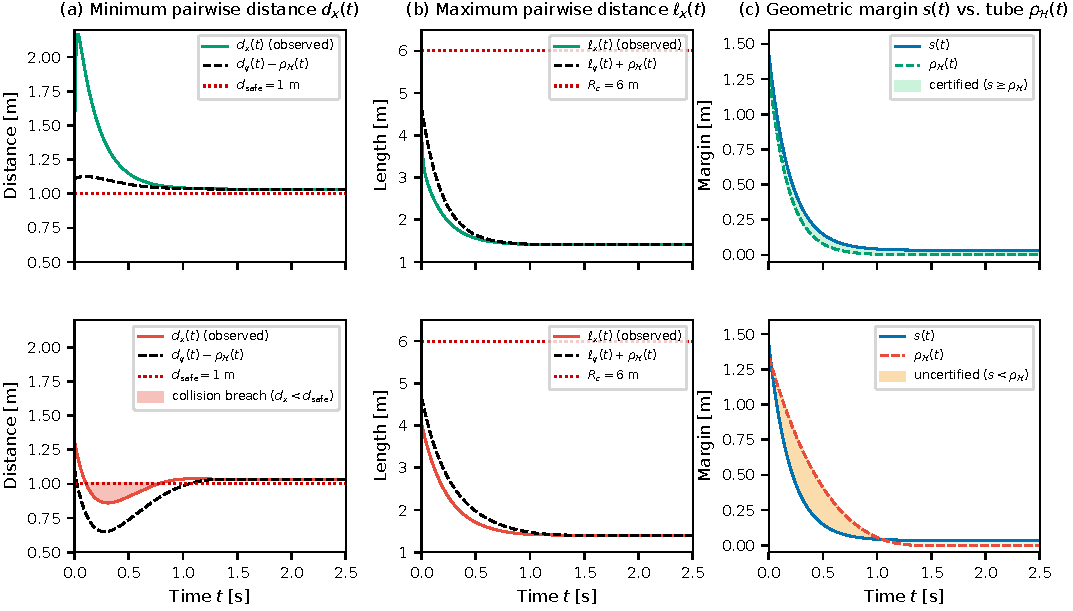
\includegraphics[width=.98\linewidth]{figures/swarm_star_2x3_comparison.pdf}
\caption{Experiment 3: Safety and connectivity during fast star compression ($\kappa=5.0$, $t \in [0, 2.5]$~s). Top row: Certified Safe ($m=30.0$). Bottom row: Unsafe Mid-Transient Collision ($m=0.0$). Columns show minimum pairwise distance $d_x(t)$ (left), maximum pairwise distance $\ell_x(t)$ (middle), and geometric margin $s(t)$ vs. distortion tube $\rho_{\mathcal{H}}(t)$ (right).}
\label{fig:star_2x3}
\end{figure}

\section{Dual expansion maneuver and transient connectivity preservation}
Complementary to rapid compression (Exp.~3), Experiment~4 tests a rapid expansion maneuver ($a_0 = 1.70 \to a_\infty = 3.02$ at $\kappa = 8.0$) to evaluate the dual physical constraint: network connectivity preservation ($\ell_x(t) \le R_c = 6.0$~m). As the star expands, nominal backbone edges stretch to $a_\infty \ell_{\mathcal{H},0} = 5.888$~m, leaving a narrow connectivity margin $s_{\rm conn}(\infty) = 0.112$~m ($11.2$~cm). The required certification rate is $\gamma_{\rm req} = 4.1367$.

\begin{table}[ht]\centering\footnotesize
\caption{Experiment 4 outcomes: Certified Safe \& Connected ($m=25.0$) vs. uncertified mid-transient disconnection ($m=0.0$) under rapid star expansion ($\kappa=8.0$, $t \in [0, 2.5]$~s).}
\begin{tabular}{@{}lrrrrrrrrrl@{}}\toprule
Case & $m$ & $\kappa$ & $\gamma$ & $\gamma_{\mathrm{req}}$ & $t_{\mathrm{set}}$ [s] & $d_{x,\min}$ & $\ell_{x,\max}$ & Peak $\|u\|$ & $J_u$ & Outcome \\\midrule
Safe & 25.0 & 8.0 & 4.8495 & 4.1367 & 0.4183 & 1.8550 & 5.8880 & 83.5699 & 3624.11 & Certified; Safe, Connected \\
Unsafe & 0.0 & 8.0 & 1.0000 & 4.1367 & 1.1333 & 1.8550 & 6.1424 & 72.3516 & 3620.46 & Uncertified; Connectivity Violation \\
\bottomrule\end{tabular}

\label{tab:star_expansion_cases}
\end{table}

Figure~\ref{fig:star_expansion_2x3} presents the corresponding $2 \times 3$ grid:
\begin{itemize}
\item \textbf{Row 1 (Certified Safe \& Connected, $m = 25.0$):} With coupling gain $m = 25.0$, $\gamma = 4.8495 > \gamma_{\rm req} = 4.1367$. All backbone communication links remain strictly within range ($\ell_{x,\max} = 5.8880\text{ m} < R_c$), and pairwise distance grows safely ($d_{x,\min} = 1.8550$~m), yielding outcome \texttt{Certified; Safe, Connected}.
\item \textbf{Row 2 (Unsafe Transient Disconnection, $m = 0.0$):} With uncoupled agents ($m = 0.0$, $\gamma = 1.0000 < \gamma_{\rm req}$), tracking lag under rapid expansion causes backbone edge stretch exceeding range: $\ell_x(t) > R_c = 6.0$~m during $t \in [0.19, 0.64]$~s (duration $0.45$~s, peak $\ell_{x,\max} = 6.1424$~m), suffering a genuine connectivity violation (\texttt{Uncertified; Connectivity Violation}).
\end{itemize}

\begin{figure}[ht]\centering
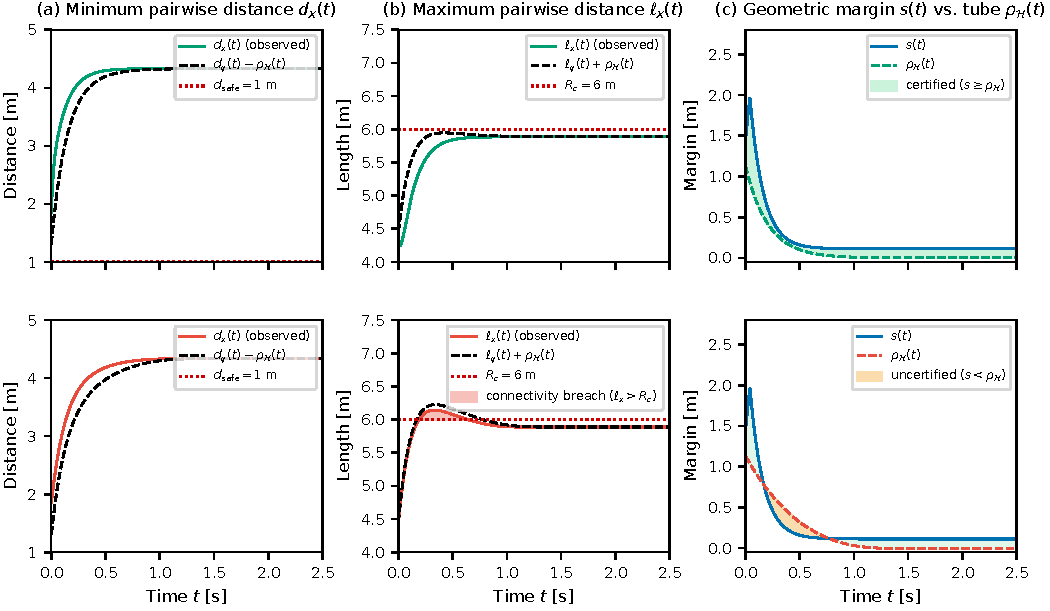
\includegraphics[width=.98\linewidth]{figures/swarm_star_expansion_2x3_comparison.pdf}
\caption{Experiment 4: Safety and connectivity during fast star expansion ($a_0 = 1.70 \to a_\infty = 3.02$, $\kappa=8.0$, $t \in [0, 2.5]$~s). Top row: Certified Safe \& Connected ($m=25.0$). Bottom row: Unsafe Transient Disconnection ($m=0.0$). Columns show minimum pairwise distance $d_x(t)$ (left), maximum pairwise distance $\ell_x(t)$ (middle), and geometric margin $s(t)$ vs. distortion tube $\rho_{\mathcal{H}}(t)$ (right).}
\label{fig:star_expansion_2x3}
\end{figure}

\section{Reproduction}
All experiments in this document can be reproduced using:
\begin{itemize}
\item Experiment 1: \texttt{python3 run\_experiments.py --experiment 1}
\item Experiment 2: \texttt{python3 run\_experiments.py --experiment 2}
\item Experiment 3: \texttt{python3 run\_experiments.py --experiment 3}
\item Experiment 4: \texttt{python3 run\_experiments.py --experiment 4}
\end{itemize}
Compile the document from \texttt{ECC\_paper/} using \texttt{pdflatex numerical\_results.tex}.
\end{document}
